\begin{figure}[t]
\centering
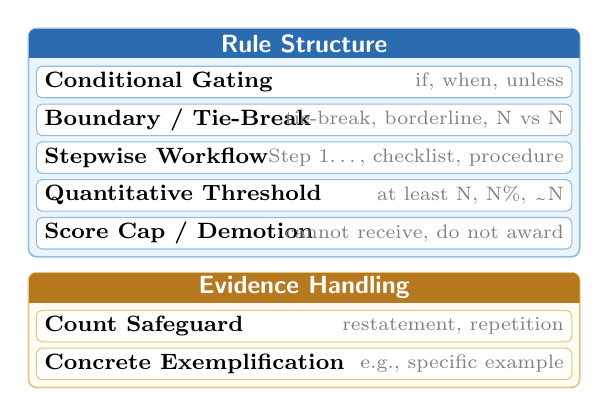
\begin{tikzpicture}[
  font=\small\sffamily,
  every node/.style={inner sep=0pt, outer sep=0pt},
]

% ── colors ──
\definecolor{RuleHdr}{HTML}{2B6CB0}
\definecolor{RuleFrame}{HTML}{90BEE0}
\definecolor{RuleBg}{HTML}{EBF4FA}
\definecolor{EvidHdr}{HTML}{B7791F}
\definecolor{EvidFrame}{HTML}{E2C97A}
\definecolor{EvidBg}{HTML}{FEFCF3}

% ── Rule Structure ──
\fill[RuleBg, rounded corners=3pt] (0.00,-2.90) rectangle (7.00,-0.00);
\draw[RuleFrame, rounded corners=3pt, line width=0.6pt] (0.00,-2.90) rectangle (7.00,-0.00);
\begin{scope}
  \clip[rounded corners=3pt] (0.00,-2.90) rectangle (7.00,-0.00);
  \fill[RuleHdr] (0.00,-0.38) rectangle (7.00,-0.00);
\end{scope}
\node[anchor=center, text=white, font=\small\bfseries\sffamily] at (3.50,-0.19) {Rule Structure};
\fill[white, rounded corners=2pt] (0.10,-0.88) rectangle (6.90,-0.48);
\draw[RuleFrame, rounded corners=2pt, line width=0.4pt] (0.10,-0.88) rectangle (6.90,-0.48);
\node[anchor=west, font=\footnotesize\bfseries] at (0.20,-0.68) {Conditional Gating};
\node[anchor=east, font={\fontsize{7.5}{9}\selectfont}, text=black!50] at (6.80,-0.68) {if, when, unless};
\fill[white, rounded corners=2pt] (0.10,-1.36) rectangle (6.90,-0.96);
\draw[RuleFrame, rounded corners=2pt, line width=0.4pt] (0.10,-1.36) rectangle (6.90,-0.96);
\node[anchor=west, font=\footnotesize\bfseries] at (0.20,-1.16) {Boundary / Tie-Break};
\node[anchor=east, font={\fontsize{7.5}{9}\selectfont}, text=black!50] at (6.80,-1.16) {tie-break, borderline, N vs N};
\fill[white, rounded corners=2pt] (0.10,-1.84) rectangle (6.90,-1.44);
\draw[RuleFrame, rounded corners=2pt, line width=0.4pt] (0.10,-1.84) rectangle (6.90,-1.44);
\node[anchor=west, font=\footnotesize\bfseries] at (0.20,-1.64) {Stepwise Workflow};
\node[anchor=east, font={\fontsize{7.5}{9}\selectfont}, text=black!50] at (6.80,-1.64) {Step 1\ldots, checklist, procedure};
\fill[white, rounded corners=2pt] (0.10,-2.32) rectangle (6.90,-1.92);
\draw[RuleFrame, rounded corners=2pt, line width=0.4pt] (0.10,-2.32) rectangle (6.90,-1.92);
\node[anchor=west, font=\footnotesize\bfseries] at (0.20,-2.12) {Quantitative Threshold};
\node[anchor=east, font={\fontsize{7.5}{9}\selectfont}, text=black!50] at (6.80,-2.12) {at least N, N\%, {\texttildelow}N};
\fill[white, rounded corners=2pt] (0.10,-2.80) rectangle (6.90,-2.40);
\draw[RuleFrame, rounded corners=2pt, line width=0.4pt] (0.10,-2.80) rectangle (6.90,-2.40);
\node[anchor=west, font=\footnotesize\bfseries] at (0.20,-2.60) {Score Cap / Demotion};
\node[anchor=east, font={\fontsize{7.5}{9}\selectfont}, text=black!50] at (6.80,-2.60) {cannot receive, do not award};

% ── Evidence Handling ──
\fill[EvidBg, rounded corners=3pt] (0.00,-4.56) rectangle (7.00,-3.10);
\draw[EvidFrame, rounded corners=3pt, line width=0.6pt] (0.00,-4.56) rectangle (7.00,-3.10);
\begin{scope}
  \clip[rounded corners=3pt] (0.00,-4.56) rectangle (7.00,-3.10);
  \fill[EvidHdr] (0.00,-3.48) rectangle (7.00,-3.10);
\end{scope}
\node[anchor=center, text=white, font=\small\bfseries\sffamily] at (3.50,-3.29) {Evidence Handling};
\fill[white, rounded corners=2pt] (0.10,-3.98) rectangle (6.90,-3.58);
\draw[EvidFrame, rounded corners=2pt, line width=0.4pt] (0.10,-3.98) rectangle (6.90,-3.58);
\node[anchor=west, font=\footnotesize\bfseries] at (0.20,-3.78) {Count Safeguard};
\node[anchor=east, font={\fontsize{7.5}{9}\selectfont}, text=black!50] at (6.80,-3.78) {restatement, repetition};
\fill[white, rounded corners=2pt] (0.10,-4.46) rectangle (6.90,-4.06);
\draw[EvidFrame, rounded corners=2pt, line width=0.4pt] (0.10,-4.46) rectangle (6.90,-4.06);
\node[anchor=west, font=\footnotesize\bfseries] at (0.20,-4.26) {Concrete Exemplification};
\node[anchor=east, font={\fontsize{7.5}{9}\selectfont}, text=black!50] at (6.80,-4.26) {e.g., specific example};

\end{tikzpicture}
\caption{\textsc{Rule Structure} patterns capture procedural and structural constraints that guide the scoring process; \textsc{Evidence Handling} patterns govern how evidence quality and quantity are assessed. Gray keywords on the right indicate the case-insensitive regular-expression triggers used to detect each pattern from the rubric text. Detailed definitions and examples of these patterns are provided in \autoref{fig:pattern_explanation} in Appendix~\ref{app:rubric_analysis}.}
\label{fig:pattern_overview}
\end{figure}